
\documentclass[10pt,a4paper]{article}

%%%%%%%%%%%%%%%%%%%%%%%%%%%%%%%%%%%%%%%%%%%%%%%%%%%%%%%%
%
% Packages and Theorem Environments

\usepackage{graphicx}
\usepackage{psfrag}
\usepackage{epsf}
\usepackage{amsmath,amsfonts,amssymb,latexsym}
\usepackage{enumitem}
\usepackage{algorithmic}
\usepackage{algorithm}
\usepackage[width=160mm,height=240mm,left=35mm,foot=10mm]{geometry}
\usepackage{xcolor}
\usepackage{url}
\usepackage{hyperref}
\usepackage{tikz}



\renewcommand{\theequation}{\thesection.\arabic{equation}}
\newcommand{\makeTiny}[1]{{\tiny #1}}
\newcommand{\work}{\tiny}
\newcommand{\ignore}[1]{}
\newcommand{\startClaims}{\setcounter{claim}{0}}
\newtheorem{theorem}{Theorem}[section]
\newtheorem{corollary}[theorem]{Corollary}
\newtheorem{lemma}[theorem]{Lemma}
\newtheorem{proposition}[theorem]{Proposition}
\newtheorem{conjecture}[theorem]{Conjecture}
\newtheorem{problem}[theorem]{Problem}
\newtheorem{question}[theorem]{Question}
\newtheorem{definition}[theorem]{Definition}
\newtheorem{task}[theorem]{Task}
\newtheorem{claim}{Claim}
\newtheorem{remark}[theorem]{Remark}
\newtheorem{observation}[theorem]{Observation}

\graphicspath{hw6}



\title{MATH 351--004 -- Assignment \#$6$\\
}

\author{Alex Iacob\\
ai9388}

\date{October 7, 2021}


%%%%%%%%%%%%%%%%%%%%%%%%%%%%%%%%%%%%%%%%%%%%%%%%%%%%%%%%
%
% Author's definitions


\newcommand{\NN}{\mathbb N}
\newcommand{\ZZ}{\mathbb Z}
\newcommand{\QQ}{\mathbb Q}
\newcommand{\RR}{\mathbb R}

\newcommand{\BB}{\mathcal B}
\newcommand{\ZT}{\mathcal Z}

\newcommand{\Cl}{\operatorname{Cl}}
\newcommand{\Bd}{\operatorname{Bd}}
\newcommand{\row}{\operatorname{row}}
\newcommand{\col}{\operatorname{col}}
\newcommand{\Span}{\operatorname{span}}
\newcommand{\convhull}{\operatorname{conv.hull}}
\newcommand{\tr}{\operatorname{tr}}

\newcommand{\diam}{\operatorname{diam}}

\begin{document}

\maketitle

\begin{center}
{\bf \large Part 2}
\end{center}

\subsection*{Problem 1 - Prove that if $v$ is a cut-vertex of a graph $G$,  then $v$ is not a cut-vertex of the complement $\bar{G}$ of $G$}
Suppose there exists two subgraphs $G_{1}  and  G_{2}$ and a cut-vertex $v$ such that $V(G) \ {v} = V(G_{1}) \bigcup V(G_{2})$. There exists a $uw$-path such that $u \in V(G_{1})$ and $w \in V(G_{2})$, then by Corollary 5.4, $v$ is a cut-vertex of $G$. Then when we take the complement there will be another vertex $y$ that will be in the $uw$ path. This leads to the $uw$ path in the complement not containing $v$ while containing $y$. Thus $v$ is not a cut-vertex in $\bar{G}$.

\subsection*{Problem 2 - Prove that a 3-regular graph $G$ has a cut-vertex if and only if $G$ has a bridge}
Forwards: A 3-regular graph has a cut-vertex if it has a bridge.\\
Suppose that $G$ is a 3-regular graph and has cut-vertex $u$. $G - u$ would create 2 or 3 connected components($G_{1}, G_{2}, (G_{3}) $) because $u$ has 3 neighbors.\\ 
3 Connected components: Each of these components much have exactly 1 neighbor of $u$.\\ 
2 Connected components: One connected component would have exactly 1 neighbor of $u$ and the other have 2 neighbors of $u$.\\
Removing the one neighbor $u$ would disconnect the graph. (Theorem 5.4 Corollary 5.4)\\
Backwards: A 3-regular graph has a bridge, then that graph has a cut-vertex\\
Suppose that $G$ is a 3-regular graph with vertices $u$ and $v$. Suppose that $uv$ is a bridge in $G$. Since $uv$ is a bridge, then either vertex $u$ or $v$ is a cut-vertex. Therefore $G$ has a cut-vertex. (Theorem 5.1)


\subsection*{\newpage Problem 3 -\\
(a) Let $G$ be a nontrivial connected graph. Prove that if $v$ is an end-vertex of a spanning tree of $G$, then $v$ is not a cut-vertex of G.\\\\
(b) Use (a) to give an alternative proof of the fact that every nontrivial connected graph contains at least two vertices that are not cut-vertices.\\\\
(c) Let $v$ be a vertex in a nontrivial connected graph $G$. Show that there exists a spanning tree of $G$ that contains all edges of $G$ that are incident with $v$.\\\\
(d) Prove that if a connected graph $G$ has exactly two vertices that are not cut-vertices, then $G$ is a path. [Recall that if a tree contains a vertex of degree exceeding 2, then $T$ has more than two end-vertices.]\\}

\begin{enumerate} [label=\alph*)]
\item Since we know that every graph has a spanning tree (Theorem 4.10), an end-vertex of a spanning tree is a leaf node. If we were to remove $v$ from the spanning tree and we observe that $G - v$ is still connected, then $v$ is not a cut-vertex, otherwise $G - v$ would be disconnected.\\
\item Since we know that every tree must have at least two leaf vertices(Theorem 4.3), using part (a) tells us that these leaf nodes are not cut-vertices.\\
\item Suppose you create a tree via BFS starting at node $v$. Since BFS visits every node individually without creating a cycle, a spanning tree can be created that contains all of the edges that are incident with $v$.\\
\item Since we have exactly 2 non-cut-vertices on $uv$ path $P$, these can only be the endpoints of $P$. Knowing this, adding another vertex to $P$ would lead to one of many cases:\\
Case 1: Added vertex $w$ has only an edge to a non-cut-vertex.$u$.\\
No issue, then $w$ becomes a leaf node and $u$ becomes a cut-vertex.\\
Case 2: Added vertex $w$ only an edge to a cut-vertex.\\
This would create a total of 3 non-cut-vertices, which would make $G$ no longer a path.\\
Case 3: Added vertex $w$ with edges to a non-cut-vertex and a cut-vertex.\\
This would create a total of 3 non-cut-vertices, which would make $G$ no longer a path.\\
Case 4: Added vertex $w$ with edges to only non-cut-vertices.\\
Adding $w$ would create a cycle, where no vertices are cut-vertices.\\
\end{enumerate}

\subsection*{\newpage Problem 4 - If a connected graph $G$ contains three blocks and $k$ cut-vertices, what are the possible values for $k$? Explain your answer.}
The amount of cut vertices we can have is the number of blocks - 1; in this case, we have at most 2 cut-vertices.
This is possible because if the amount of blocks equaled to the number of blocks, then the cut vertices of each block would make a cycle, which would not make them cut-vertices.
Since we have 3 blocks and a max of 2 cut vertices, we have a total of 3 possible cases:\\
2 cut-vertices:\\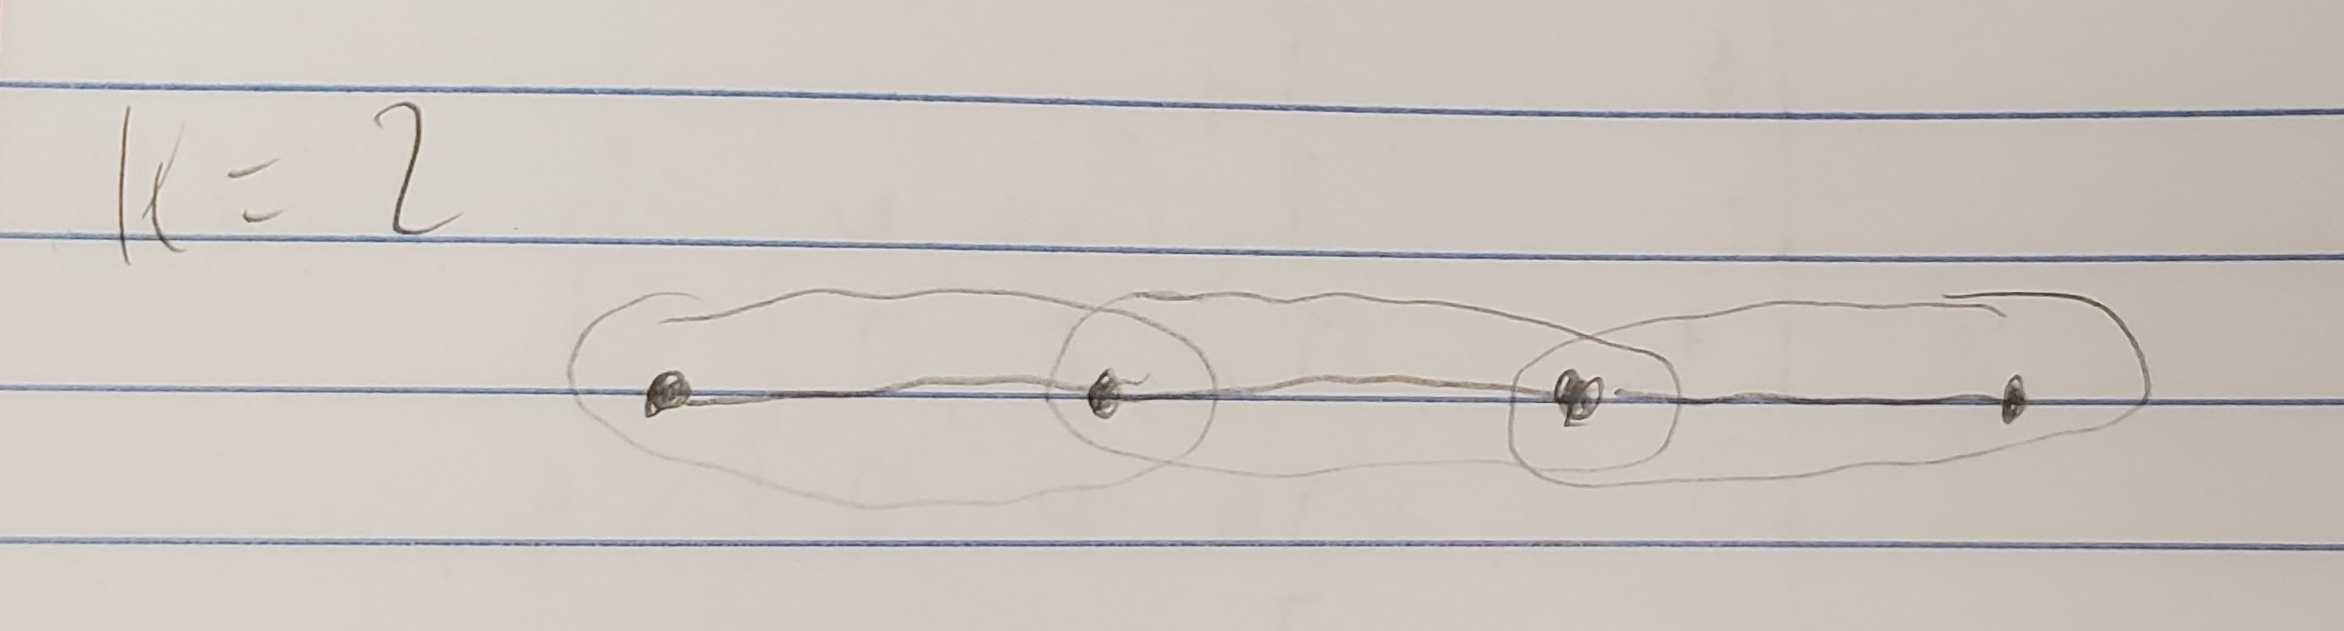
\includegraphics[width = 10cm]{k=2}\\
1 cut-vertex:\\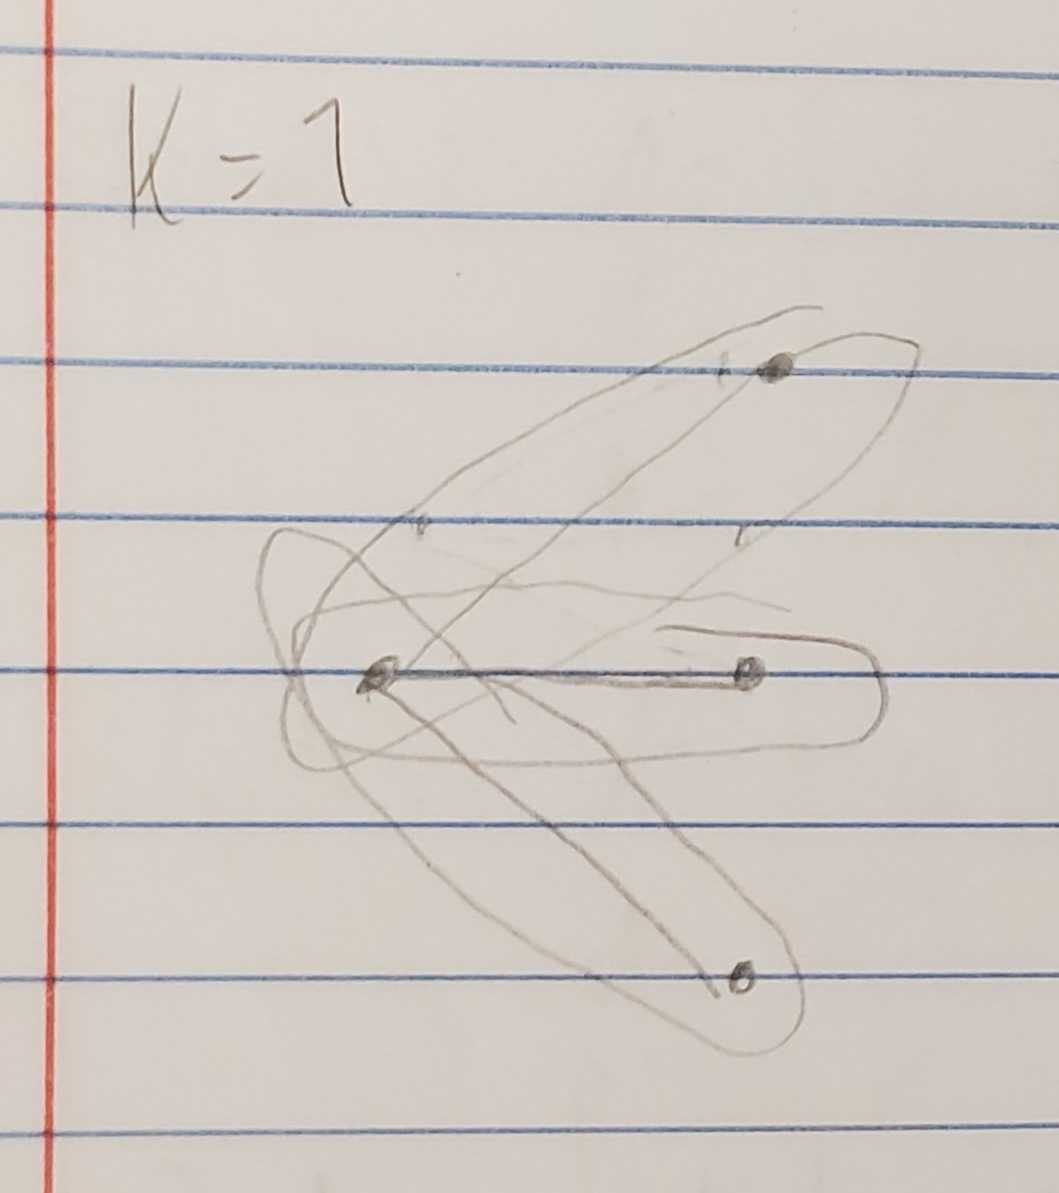
\includegraphics[width = 5cm]{k=1}\\
0 cut-vertices:\\Since $G$ is connected, and there are 3 blocks, then at least two of the blocks would have a cut-vertex in common, having 0 cut-vertices would make $G$ disconnected. \\

\end{document} 	